\newcommand{\dvm}{DVM841}
\newcommand{\vell}{Vellemann\textsuperscript{\tiny\textregistered}}

\chapter{Misura di resistenze con un multimetro digitale}\label{ch:mult}
    \lettrine[loversize=0.08, lines=2]{T}{ra le esperienze} svolte con il multimetro digitale riporto la misura delle resistenze di vari oggetti, tra cui un anello e alcuni resistori, misurati sia individualmente che in parallelo.

    Ai resistori dedico una sezione più approfondita in quanto ho preso \num{50} misure su resistori distinti---ma teoricamente con resistenza uguale---per verificare la distribuzione delle misure.

    \section{Il multimetro}
        Lo strumento utilizzato per l'interezza dell'esperienza è un multimetro digitale della serie \dvm\ della \vell\ \cite{velleman-dvm841}, \figref{fig:mul:multimetro}. Il multimetro è in grado di misurare tensione e corrente continua e alternata, resistenza, frequenza e temperatura. Avendo una risoluzione di \num{2000} punti, il display del multimetro può visualizzare un massimo di \num{1999} unità.
        \begin{figure}
            \centering
            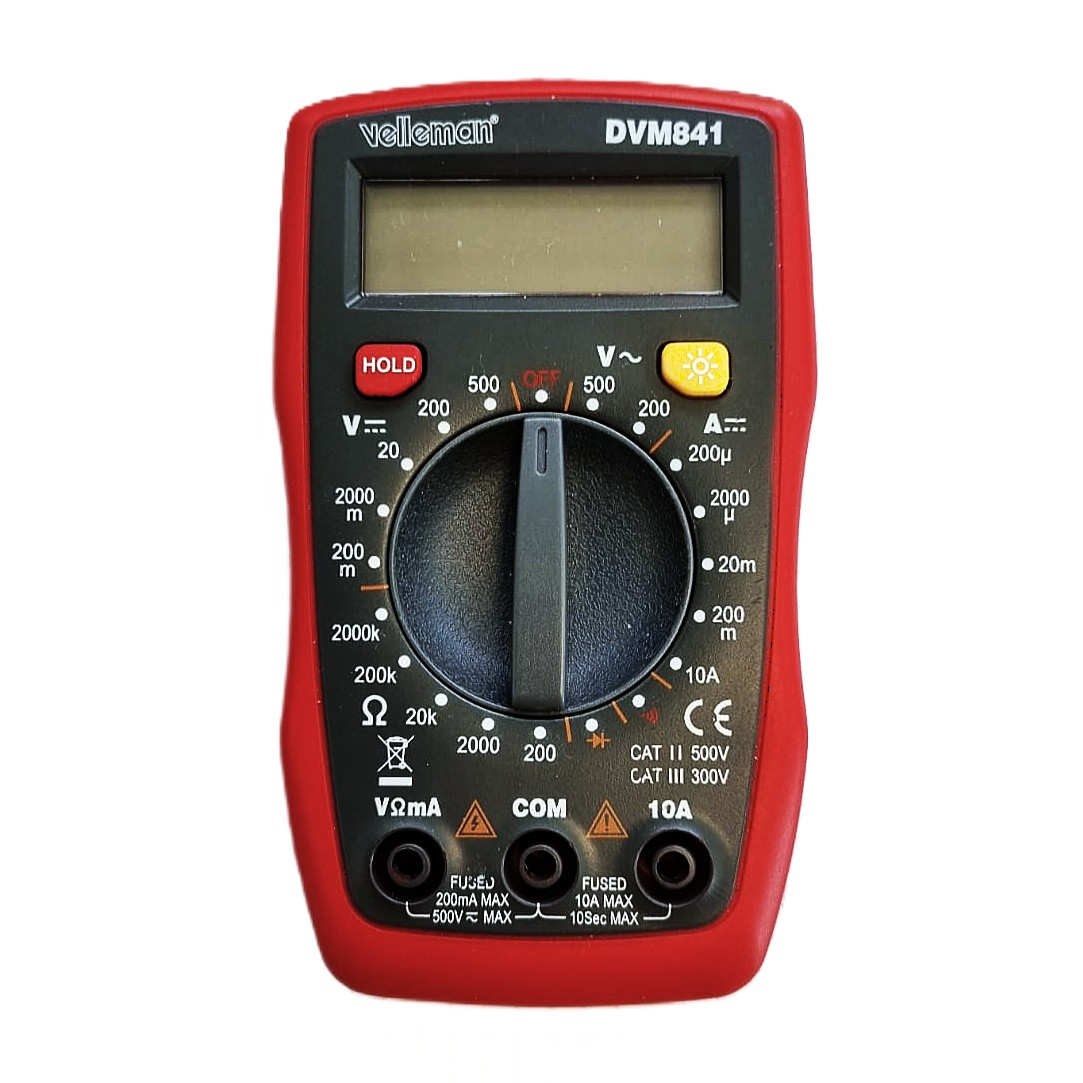
\includegraphics[width = 0.4\textwidth]{images/multimetro/multimetro.jpg}
            \caption{Il multimetro \dvm\ della \vell\ usato per l'esperienza.}
            \label{fig:mul:multimetro}
        \end{figure}

        L'apparecchio è alimentato a batteria e presenta tre prese a cui si possono collegare due puntali con gli appositi spinotti. Volendo misurare solo resistenze, ho usato solo la presa \unit{\volt\ohm\milli\ampere} e la messa a terra.

    \section{Resistori}\label{s:mul:resistori}
        Il kit presenta $N = \num{50}$ resistori distinti---come quelli in \figref{fig:mul:resistore}---il cui codice colore restituisce un valore\footnote{Lo si può dedurre da qualunque legenda fedele allo standard IEC 60062.} teorico di $\SI{820}{\ohm} \pm \SI{5}{\%}$, ovvero \SI{820(40)}{\ohm}.
        \begin{figure}
            \centering
            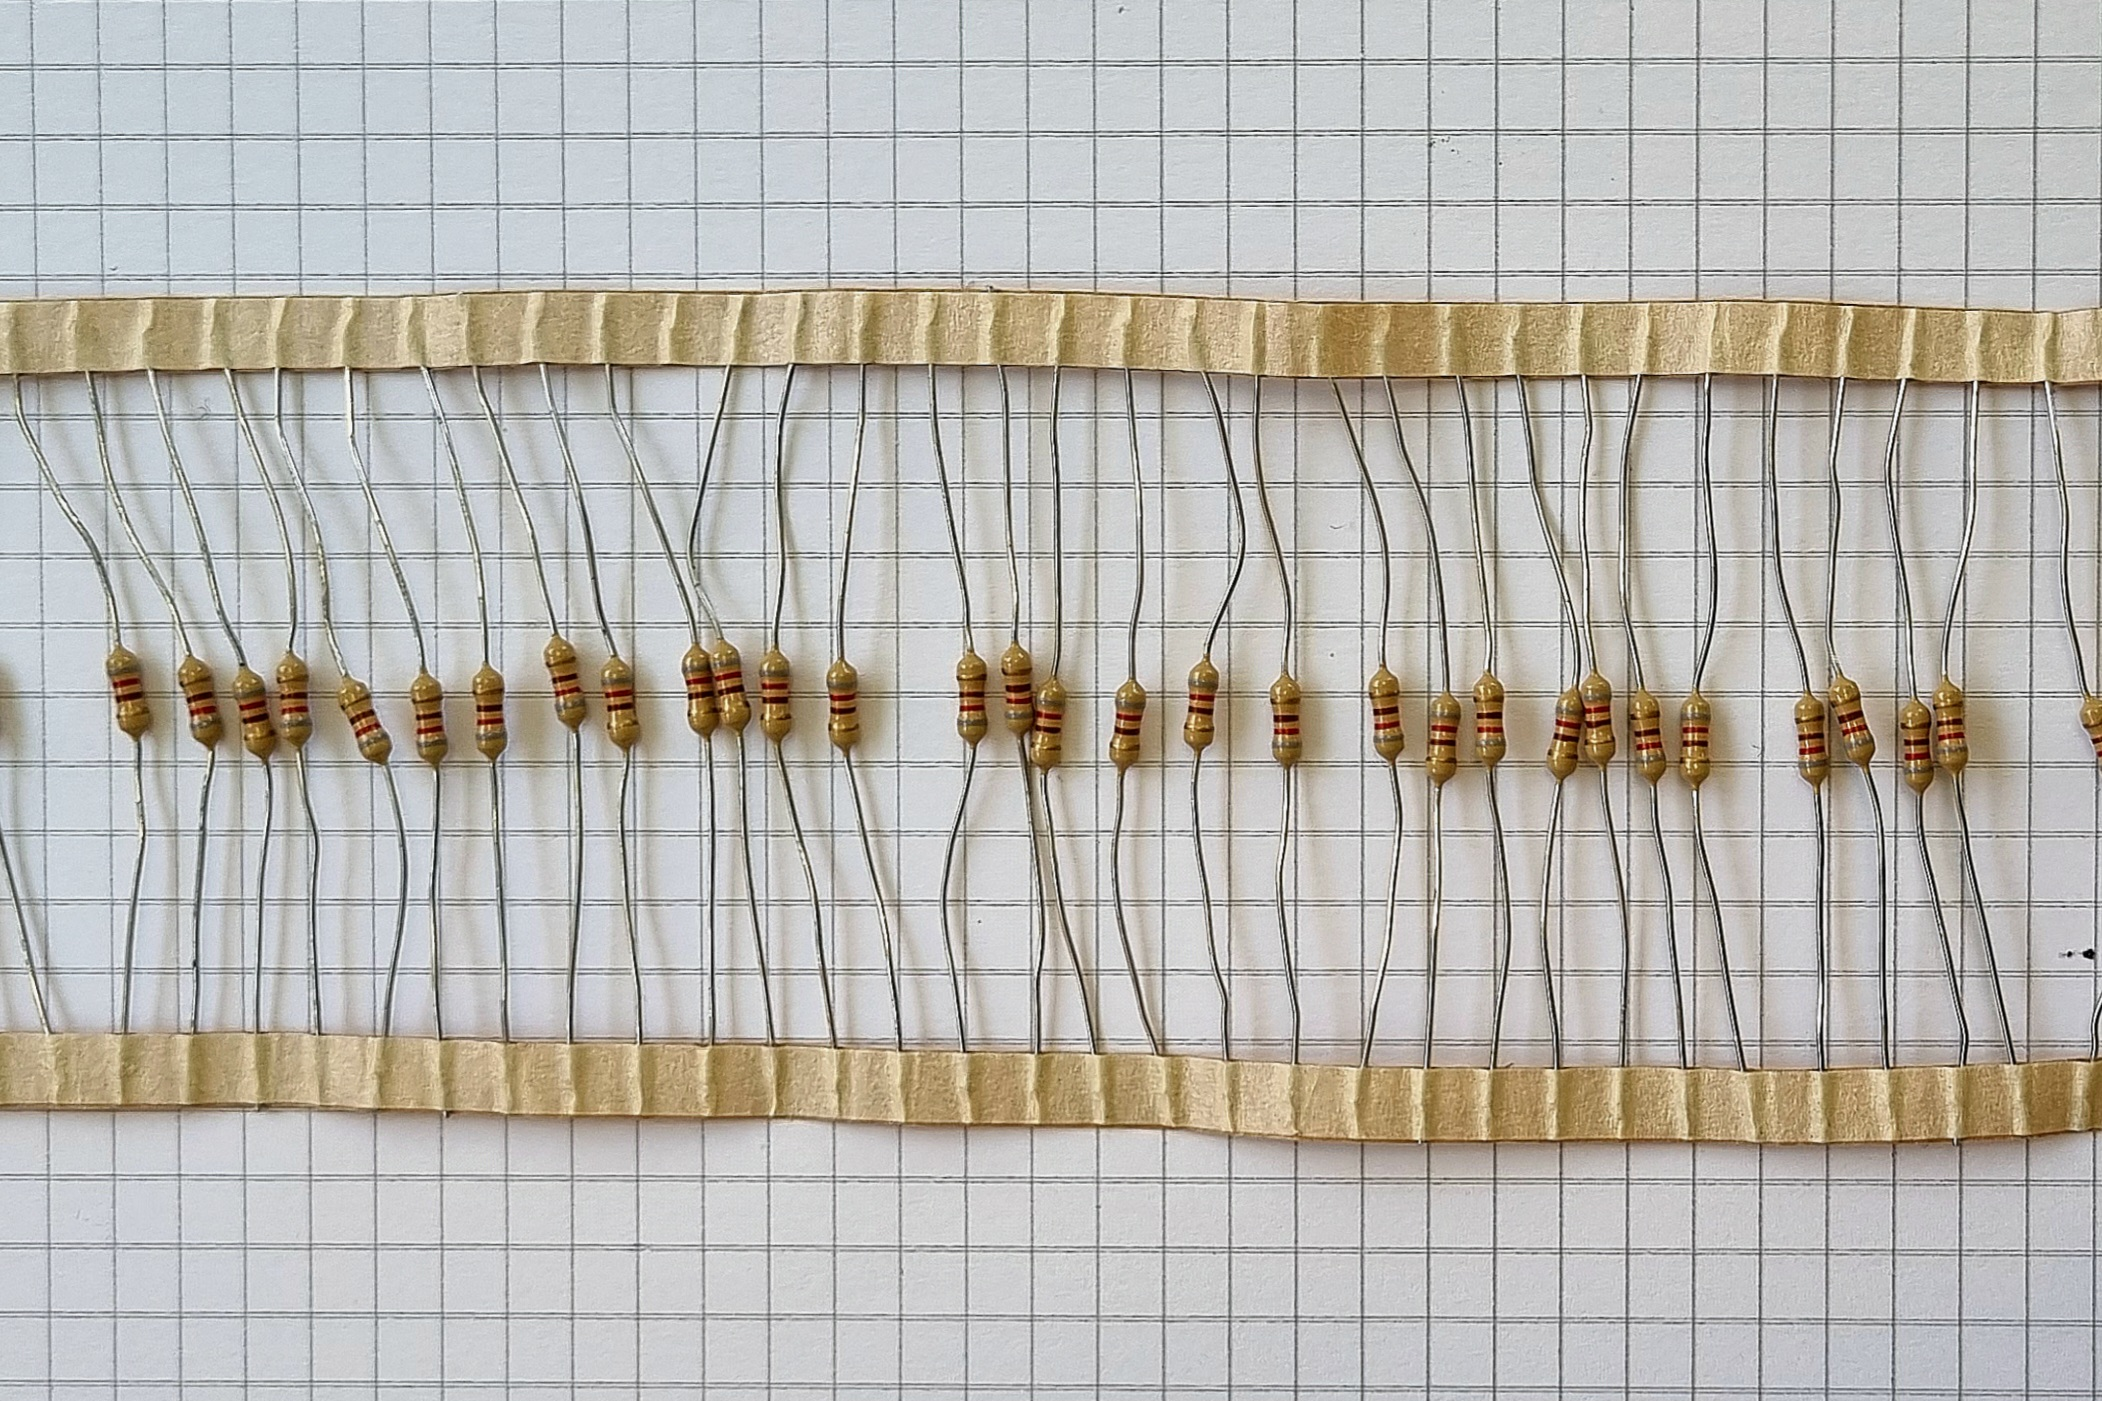
\includegraphics[width=0.4\textwidth]{images/multimetro/resistori.jpg}
            \hspace{0.05\textwidth}
            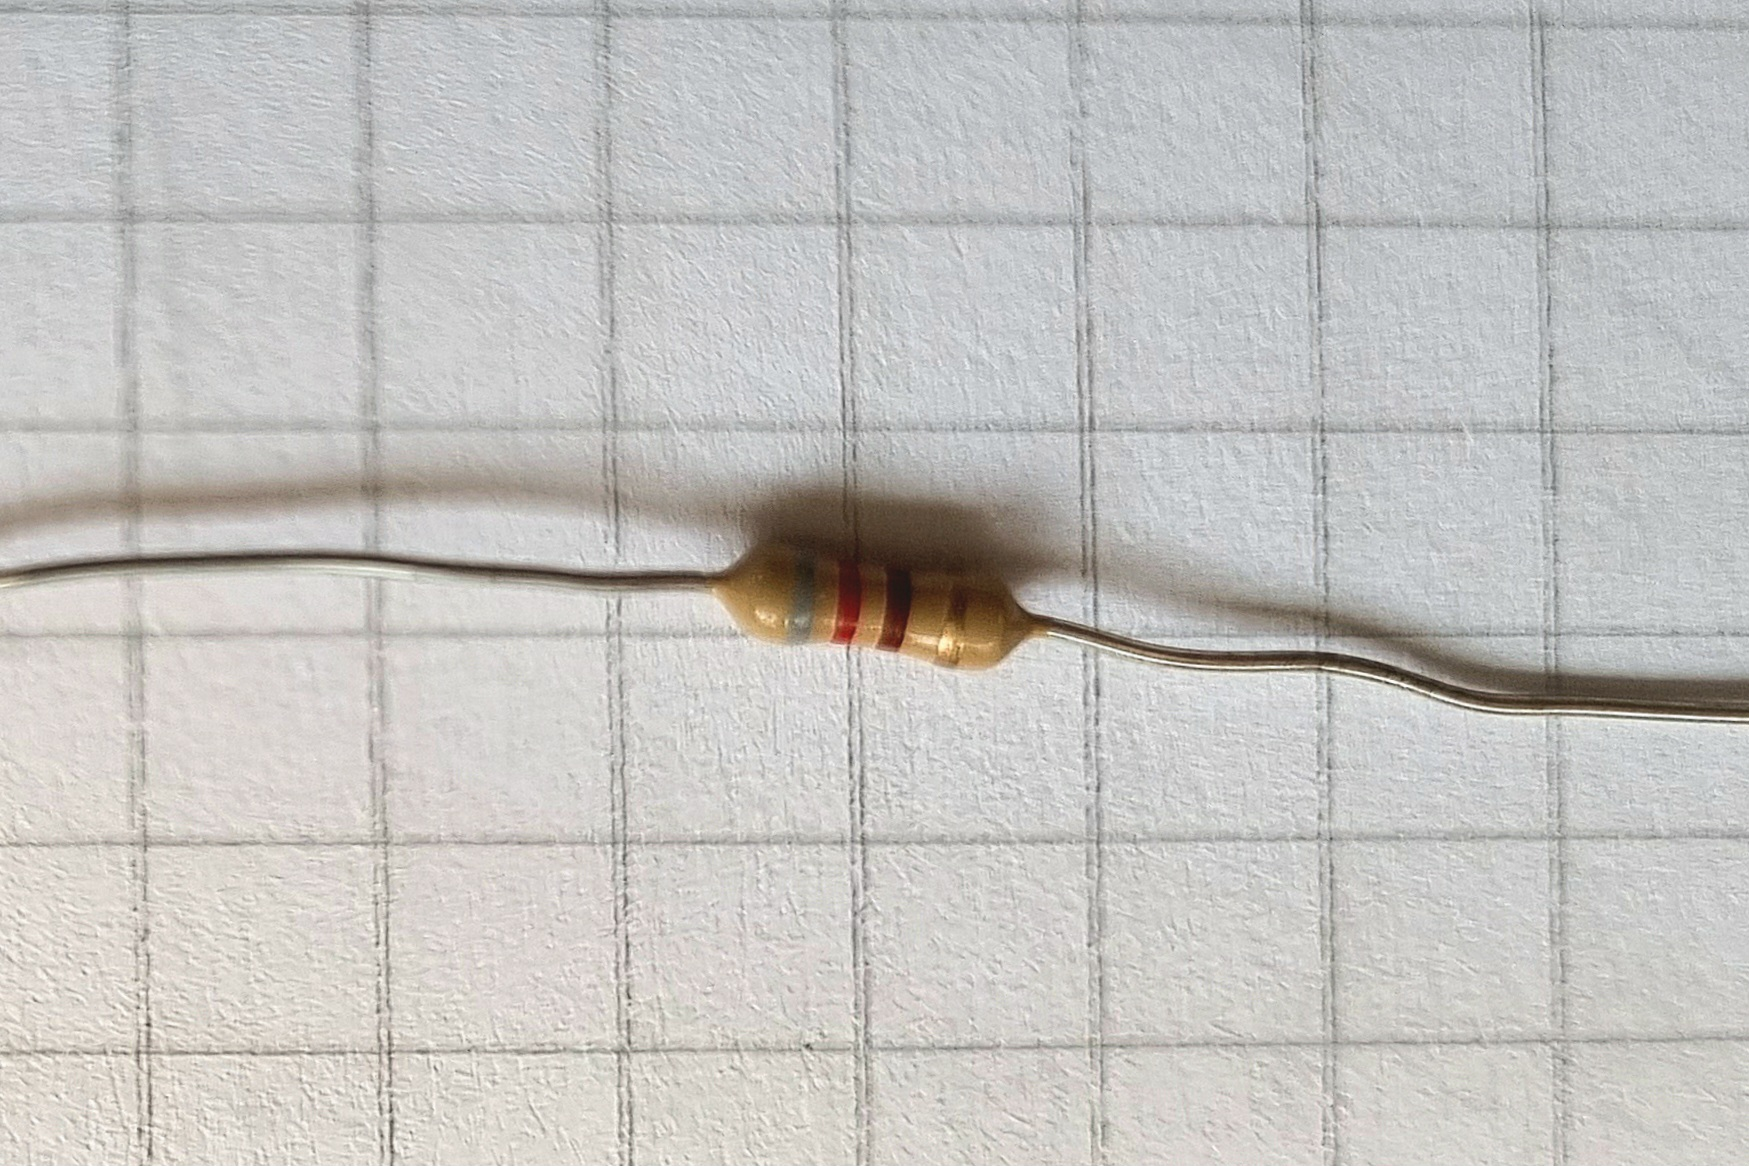
\includegraphics[width=0.4\textwidth]{images/multimetro/resistore.jpg}
            \caption{A sinistra alcuni dei \num{50} resistori da \SI{820}{\ohm}. A destra un dettaglio dove è visibile il codice colore.}
            \label{fig:mul:resistore}
        \end{figure}

        Ho effettuato le misure impostando il multimetro in modalità \emph{ohm}, alla portata di \SI{2}{\kilo\ohm}, poggiando i puntali sui terminali di ciascun resistore e aspettando di volta in volta che la lettura si stabilizzasse. I dati raccolti sono riportati in ordine crescente in \tabref{tab:mul:resistori}.
        \begin{table}
            \centering
            \begin{tabular}{cccccccccc}
    \hline
    \multicolumn{10}{c}{Resistenze (\unit{\ohm})}\\\hline\hline
    797 & 806 & 806 & 807 & 807 & 807 & 807 & 807 & 807 & 807 \\
    807 & 808 & 808 & 808 & 808 & 808 & 808 & 808 & 808 & 808 \\
    808 & 808 & 808 & 809 & 809 & 809 & 809 & 809 & 809 & 809 \\
    809 & 809 & 809 & 809 & 809 & 809 & 810 & 810 & 810 & 810 \\
    810 & 810 & 810 & 811 & 811 & 812 & 812 & 812 & 812 & 813 \\ \hline
\end{tabular}
            \caption{Misure di resistenza effettuate su \num{50} resistori distinti.}
            \label{tab:mul:resistori}
        \end{table}

        \subsection{Considerazioni preliminari}
            Notiamo subito che la resistenza media è $R_\text{m} = \SI{808.6}{\ohm}$ con una deviazione standard di $\sigma = \SI{2.3}{\ohm}$; l'errore sul valor medio è quindi $\sigma_R = \sigma / \sqrt{N-1} = \SI{0.33}{\ohm}$, che è confrontabile con la sensibilità dello strumento $\delta R_\text{s} = \SI{1}{\ohm}$.
            
            Questi valori rientrano completamete nell'intervallo fornito dal costruttore; tuttavia, il fatto che tutte le misure siano inferiori a \SI{820}{\ohm} suggerisce la presenza di un errore sistematico.\footnote{Se si trattasse di errori casuali dovuti a imprecisioni di fabbricazione, mi aspetterei letture sia al di sopra che al di sotto del valore di riferimento; è poco probabile che tutte le resistenze devino dal valore teorico allo stesso modo a meno che non si sia verificato un evento che ha alterato tutte le resistenze---un lotto prodotto con lo stesso materiale meno resistente, seppur entro il margine del \SI{5}{\%}, o deterioramento nel tempo.}

            Il dato di resistenza minima di \SI{797}{\ohm} può essere scartato secondo il cirerio di Chauvenet. Esso dista più di $4\sigma$ dal valor medio (ca. $\num{4.17}\sigma$) e il numero di dati atteso\footnote{Per il calcolo di questa probabilità ho fatto riferimento a [INSERIRE TAYLOR!!!]} su un campione di $N = 50$ elementi a una distanza maggiore o uguale a $4\sigma$ è pari a $\num{0.003} \ll 1/2$. Scartando questo dato la nuova media e la nuova deviazione standard sono:
            \begin{equation*}
                R_\text{m} = \SI{808.8}{\ohm}
                \qquad
                \sigma = \SI{1.633}{\ohm}
                \myperiod
            \end{equation*}
            La nuova incertezza sul valor medio è $\sigma_R = \SI{0.24}{\ohm} \lesssim \delta R_\text{s} = \SI{1}{\ohm}$, che è ancora confrontabile con la sensibilità dello strumento. Se tuttavia consideriamo la somma in quadratura delle due incertezze troviamo
            \begin{equation*}
                \overline{\sigma}
                = \sqrt{\sigma_R^2 + \delta R_\text{s}^2}
                = \SI{1.02}{\ohm}
                \simeq \SI{1}{\ohm}
                \mycomma
            \end{equation*}
            per cui assumo $\overline{\sigma} = \SI{1}{\ohm}$ come incertezza sul valor medio.

        \subsection{Test del $\chi^2$}
            Supponiamo che le misure seguano, con una significatività $\alpha = \num{0.05}$, la distribuzione normale centrata in $R_\text{m}$ e di ampiezza $\sigma$:
            \begin{equation*}
                N\pqty{x; R_\text{m}, \sigma}
                = \frac{1}{\sqrt{2\pi\sigma^2}} \exp[ -\frac{1}{2}\pqty{\frac{x - R_\text{m}}{\sigma}}^2]
                \myperiod
            \end{equation*}
            
            Costruiamo quindi un istogramma dei dati. Visto l'intervallo contenuto in cui le misure variano, ho scelto di raccogliere i dati in bin di ampiezza \SI{1}{\ohm}, uno per ciascun valore misurato; ciascun bin si estende da mezza unità \emph{prima} del valore di interesse a mezza unità \emph{dopo}. In \tabref{tab:mul:bin-istogramma} sono riportati i bin e le frequenze osservate $O_k$.
            \begin{table}
                \centering
                \begin{tabular}{ccccc|rc}\hline
    \multicolumn{5}{c}{Intervalli}                  & $O_k$    & $E_k$       \\
    \hline\hline
                  &     & $R$ & $<$ & $\num{806.5}$ & \num{2}  & \num{4.133} \\
    $\num{806.5}$ & $<$ & $R$ & $<$ & $\num{807.5}$ & \num{8}  & \num{5.735} \\
    $\num{807.5}$ & $<$ & $R$ & $<$ & $\num{808.5}$ & \num{12} & \num{6.925} \\
    $\num{808.5}$ & $<$ & $R$ & $<$ & $\num{809.5}$ & \num{13} & \num{7.278} \\
    $\num{809.5}$ & $<$ & $R$ & $<$ & $\num{810.5}$ & \num{6}  & \num{6.655} \\
    $\num{810.5}$ & $<$ & $R$ & $<$ & $\num{811.5}$ & \num{2}  & \num{5.297} \\
    $\num{811.5}$ & $<$ & $R$ & $<$ & $\num{812.5}$ & \num{4}  & \num{3.668} \\
    $\num{812.5}$ & $<$ & $R$ &     &               & \num{1}  & \num{2.211} \\
    \hline
\end{tabular}
                \caption{Suddivisione dei dati per il test del $\chi^2$. Ometto le unità di misura per chiarezza espositiva e semplicità dei calcoli.}
                \label{tab:mul:bin-istogramma}
            \end{table}

            Nella stessa tabella sono riportati i valori attesi $E_k$ per ciascun bin, calcolati moltiplicando la dimensione del campione $N = 49$ per l'integrale di ciascun intervallo della gaussiana. Ho ottenuto gli intervalli convertendo gli estremi in variabili normali standardizzate e ho ricavato l'integrale attraverso un foglio di calcolo.

            È adesso possibile calcolare il $\chi^2$ per definizione:
            \begin{equation*}
                \chi^2
                = \sum_{k=1}^{8} \frac{(O_k - E_k)^2}{E_k}
                = \num{12.98}
                \myperiod
            \end{equation*}
            essendo $d = n - c = 6$ il numero di gradi di libertà, $n = 8$ il numero di bin e $c = 2$ il numero di parametri stimati---media e deviazione standard. Il valore critico per il test del $\chi^2$ è $\chi^2_\text{crit}= \num{12.59}$ \cite{chi2-table}, posso quindi rigettare l'ipotesi nulla che le misure seguano la distribuzione gaussiana.

    \section{Altre misure di resistenze}
        Riporto altre misure eseguite con il multimetro su vari materiali.
        
        \subsection{Resistenze in parallelo}
            Usando $n = 1, 2, 3$ resistori scelti casualmente tra quelli studiati al punto \Sref{s:mul:resistori}, ho misurato la resistenza equivalente $R_\text{o}$ dei resistori montati in parallelo su una breadboard come in \figref{fig:mul:res-parallelo}. I risultati sono riportati in \tabref{tab:mul:res-parallelo}, insieme ai valori teorici, calcolati a partire dalla $R_\text{m}$ del punto precedente come
            \begin{equation*}
                \frac{1}{R_\text{e}}
                = \frac{n}{R_\text{m}}
                \iff R_\text{e} = \frac{R_\text{m}}{n}
                \mycomma
            \end{equation*}
            e alle incertezze $\delta R_\text{s}$ e $\delta R_\text{e}$. La prima è ancora la sensibilità dello strumento, mentre la seconda è calcolata propagando l'incertezza $\overline{\sigma}$ sul valor medio $R_\text{m}$ trovata al punto \Sref{s:mul:resistori}:
            \begin{equation*}
                \delta R_\text{e}
                = \abs{\pdv{R_\text{e}}{R}}\overline{\sigma}
                = \frac{\overline{\sigma}}{n}
                \mycomma
            \end{equation*}
            \begin{figure}
                \centering
                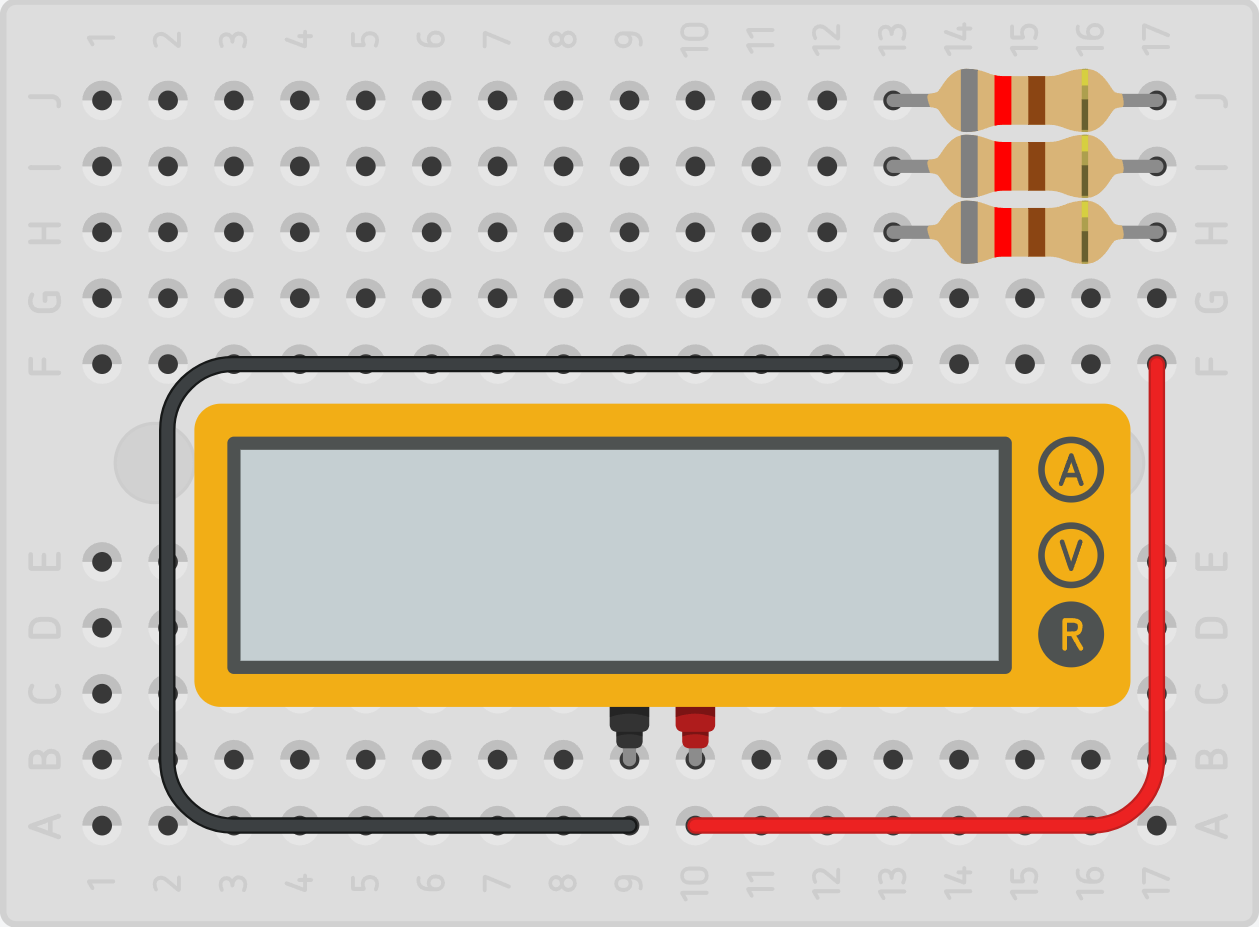
\includegraphics[width=0.4\textwidth]{images/multimetro/res-parallelo.png}
                \caption{Illustrazione rappresentativa dei resistori montati in parallelo su una breadboard.}
                \label{fig:mul:res-parallelo}
            \end{figure}
            \begin{table}
                \centering
                \begin{tabular}{ccccc}
    \hline
    $n$ & $R_\text{o}$   & $\delta R_\text{s}$  & $R_\text{e}$  & $\delta R_\text{e}$ \\
    \hline\hline
    $1$ & \num{815}      & \num{1}              & \num{808.8}   &  \num{1}            \\
    $2$ & \num{410}      & \num{1}              & \num{404.4}   &  \num{0.5}          \\
    $3$ & \num{272}      & \num{1}              & \num{269.6}   &  \num{0.3}          \\
    \hline
\end{tabular}
                \caption{Resistenze equivalenti misurate su resistori in parallelo e relative incertezze. Tutti i valori sono espressi in \unit{\ohm}.}
                \label{tab:mul:res-parallelo}
            \end{table}

            Osservando i dati si nota che la resistenza equivalente osservata $R_\text{o}$ è sempre maggiore della resistenza teorica $R_\text{e}$. Questo può essere dovuto alla presenza di una resistenza di contatto con la breadboard, che non ho considerato nel calcolo di $R_\text{e}$.

        \subsection{Resistività di un anello}
            Ho misurato la resistenza di un anello metallico che suppongo essere in argento. L'anello è di forma circolare ma presenta un'apertura in basso, per cui ho effettuato la misura della resistenza poggiando i puntali del multimetro in corrispondenza dei punti estremi dell'apertura, come in \figref{fig:mul:anello}. Ho posto il multimetro alla portata di \SI{200}{\ohm} disponendo di una sensibilità $\delta R_\text = \SI{0.1}{\ohm}$; la resistenza misurata è quindi $R = \SI{0.5}{\ohm}$.

            Dalla seconda legge di Ohm possiamo ricavare la resistività del materiale che compone l'anello, supponendo che esso sia omogeneo e isotropo. La resistività è definita come
            \begin{equation}
                \rho = R\frac{S}{L}
                \mycomma
                \label{eq:mul:ohm-law}
            \end{equation}
            dove $S$ è la sezione dell'anello e $L$ la lunghezza equivalente ottenuta rettificando la circonferenza.
            \begin{figure}
                \centering
                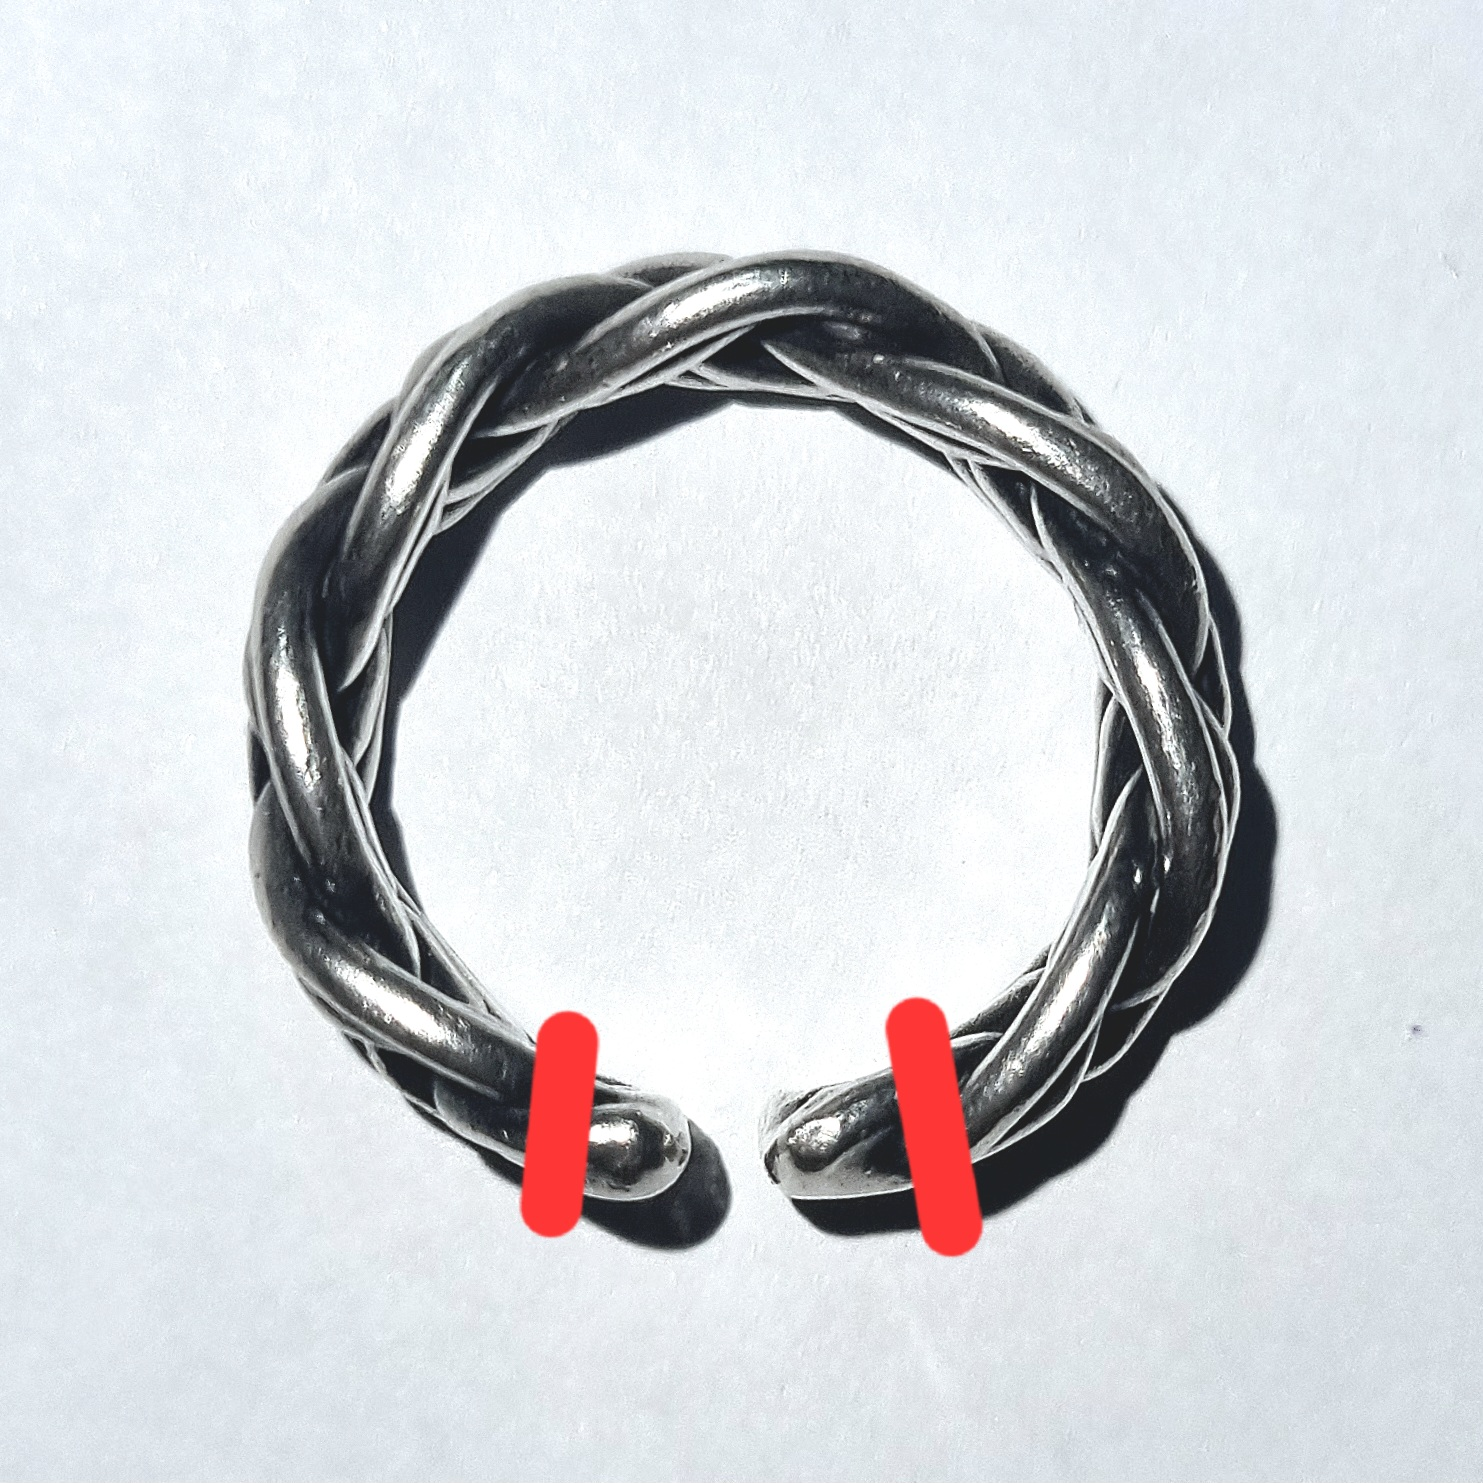
\includegraphics[width=0.4\textwidth]{images/multimetro/anello.jpg}
                \caption{Fotografia dell'anello. I tratti in rosso indicano il punti in cui sono stati poggiati i puntali del multimetro.}
                \label{fig:mul:anello}
            \end{figure}

            L'anello ha una raggio medio di $r = \SI{2.1(1)}{\centi\meter}$, uno spessore di $d = \SI{0.3(1)}{\centi\meter}$ e un'altezza pari a $h = \SI{0.8(1)}{\centi\meter}$. La sezione dell'anello è quindi $S = hd = \SI{0.24(11)}{\centi\meter\squared}$, mentre, denotando con $\ell = \SI{1.0(1)}{\centi\meter}$ la distanza che separa i due puntali e che quindi non partecipa alla resistenza, la lunghezza equivalente è $L = 2\pi r - \ell = \SI{12.3(7)}{\centi\meter}$.

            Dal momento che l'anello è formato da fili cilindrici intrecciati, la sezione $S$ rappresenta in realtà una sovrastima della sezione effettiva. Il rapporto tra la superficie di un cerchio di raggio $d/2$ e quella di un quadrato di lato $d$ è pari a $\pi / 4$, per cui la sezione effettiva è $S_\text{eff} = S \pi / \num{4} = \SI{0.19(8)}{\centi\meter\squared}$.
            
            La resistività dell'anello calcolata dalla \eqref{eq:mul:ohm-law} è quindi
            \begin{equation*}
                \rho = R\frac{S_\text{eff}}{L} = \SI{0.0077(55)}{\ohm\centi\meter} = \SI{7.7(55)e-5}{\ohm\meter}
                \mycomma
            \end{equation*}
            valore che si discosta di diversi ordini di grandezza da quello noto di \SI{1.59e-8}{\ohm\meter} \cite{Griffiths2012-qz}. Un risultato così elevato può essere attribuito sia all'incertezza sulle misure geometriche, sia al fatto che l'anello non sia composto da argento puro, sia alla presenza di ossidazione superficiale o di cattivi contatti tra i fili intrecciati che ne aumentano la resistenza complessiva.
            


